% !TeX encoding = utf8
%
%*******************************************************
% Construcción redes neuronales  una capa 
%*******************************************************
% Introducción al capítulo 

A lo largo de este capítulo daremos una modelización propia de red  neuronal y la compararemos con otros modelos ofrecidos.
Probaremos además que el modelo propuesto es un aproximador universal, es decir es capaz de aproximar cualquier función medible. 


% Comienzo de la sección 
\section{Definición de las redes neuronales \textit{Feedforward Networks} 
de una capa oculta} \label{sec:redes-neuronales-intro-una-capa}

Ya estamos en condiciones de introducir qué es una red neuronal,
cómo está construida y en qué consiste el \textit{aprendizaje} de la misma. 
Concretamente
construiremos el tipo particular \textit{Feedforward Neural Networks}, al cual nos referiremos de ahora
en adelante como red neuronal.

De acorde con nuestra filosofía de trabajo expuesta en la introducción del capítulo \ref{motivo-una-capa}
partiremos de un modelo de una sola capa oculta y además comenzaremos presentando el modelo que 
hemos considerado más conveniente; esta decisión es argumentada en el capítulo \ref{chapter:construir-redes-neuronales}. 

% Imagen grafo red neuronal  una capa oculta muy simple y en blanco y negro 
\begin{figure}[h!]
    \centering
    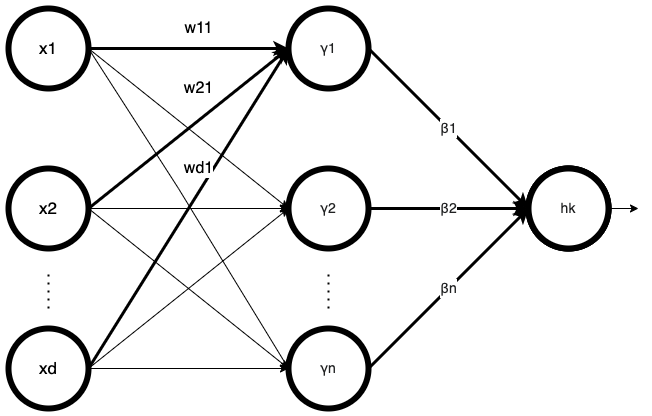
\includegraphics[width=0.85\textwidth]{1-Introduccion_redes_neuronales/Red-Neuronal-una-capa-simple.png}
    \caption{\textit{Grafo} de una red neuronal de una capa oculta}
    \label{img:grafo-red-neuronal-una-capa-oculta}
\end{figure}

    \begin{aportacionOriginal}
    \begin{definicion}[Redes neuronales de una capa oculta] \label{definition:redes_neuronales_una_capa_oculta}
        Dados $X \subseteq \R^d, Y \subseteq \R^s$ y  $\Gamma$ un conjunto no vacío de funciones medibles definidas de $\R$ a $\R$, denotaremos como 
        \begin{align}
            \mathcal{H}(X,Y) 
            =
            \{
                h : X \longrightarrow Y 
                /& \quad 
                h_k(x) = 
                \sum_{i=1}^{n} \beta_{i k} \gamma_{i}( A_{i}(x)), \\
                & \text{donde  $h_k$  es la proyección k-ésima de $h$ con 
                $k \in \{1, \ldots, s\}$}, \\
                & n \in \N,\gamma_{i} \in \Gamma , \beta_{i k} \in \R
                \text{ y }A_{i} \text{ una aplicación afín de $\R^d$ a $\R$}           
            \}.
        \end{align}
    \end{definicion}
\end{aportacionOriginal}

% Nota margen aclarativa de una función medible
\reversemarginpar
\setlength{\marginparwidth}{\smallMarginSize}
\marginpar{\maginLetterSize
    \iconoAclaraciones \textcolor{dark_green}{     
        \textbf{Qué son las funciones medibles 
        y porqué las usamos en nuestra definición.}
    }
    {\maginLetterSize
        A nivel intuitivo una función medible es aquella,
        que por muy extraña que sea
        su imagen (los valores que toma su salida) está acotada casi siempre, lo que a nivel práctico 
        significa que \textit{podemos observar y cuantificar sus valores.}
    
        Con esto pretendemos que nuestra definición $\Gamma$ 
        sea lo menos restrictiva posible.
    }
}
\normalmarginpar
\setlength{\marginparwidth}{\bigMarginSize}

% Nota margen aclarativa de la fórmula
\marginpar{\maginLetterSize
    \iconoAclaraciones \textcolor{dark_green}{     
        \textbf{Interpretación fórmula}
    }
    {\maginLetterSize
        Observemos que $n$ es el número de neuronas de la capa oculta. Es decir lo que en el grafo \ref{img:grafo-red-neuronal-una-capa-oculta} serían las neuronas de las capas ocultas se correspondería con términos $\gamma_{i}( A_{i}(x))$.
    }
}
\normalmarginpar
\setlength{\marginparwidth}{\bigMarginSize}


Es habitual representar una red neuronal de forma matricial, veremos que tal forma es equivalente a la definición dada. 

Consideramos la aplicación inclusión 
$i: \R^r \longrightarrow \R^{r+1}$ dada por 
 $i((x_1, \ldots, x_d)) = (1,x_1, \ldots, x_d).$
Para coeficientes $w_i \in \R$ toda función afín es de la forma 
$A_{i}(x)= \sum_{j=1}^d( w_{j i} x_j) + w_{0i}$, 
tomando $W_i = (w_{0 i}, w_{1 i}, \ldots, w_{r i}) \in \R^{r+1}$ tenemos que 
$A_i(x) = W_i \cdot i(x)$ como queríamos probar. 

Además también se suele mostrar de manera pedagógica con un grafo como el mostrado en la 
figura \ref{img:grafo-red-neuronal-una-capa-oculta}.

% Elimino TODO porque ya se ha comentado.

\subsection*{Componentes de la red neuronal}  

A la vista de la definición dada notemos que cada elemento de 
$\mathcal{H}(X,Y)$ viene determinado por los coeficientes 
de las distintas $\beta$ y  $w$s de la función afín. Como veremos más adelante estos son los valores que \textit{aprende una red neuronal}.

\subsection*{Diferencia con otras definiciones}  \label{subsection:diferencia-otras-definiciones-RRNN}

En otros textos como en el capítulo cinco, páginas 227-256 del libro \cite{BishopPaterRecognition} y las notas online sobre redes neuronales de \cite{MostafaLearningFromData} se presentan las redes neuronales de una capa como 
\begin{align}
    y_k(x,w) &= \theta_k 
    \left( 
        \sum^M_{j=1} w_{ji}^{(2)}
        \sigma_j 
        \left(
            \sum_{i=1}^D w_{ji}^{(1)} x_i + w_{j0}^{(1)}
        \right)
        + w_{k0}^{(2)}
    \right) 
    \\
    & = 
    \theta_k 
    \left( 
        \sum^M_{j=1} A^{(n_k)}_{k}
        \left(
            \sigma 
            \left(
                A^{r}_{j k}
                \left(
                    x
                \right)
            \right)
        \right)
    \right)
    \text{ para cada  } k \in \{1, \ldots, K \}.
\end{align}

Donde $\theta_k$ representa una función de \textit{clasificación}, 
$\sigma_j$ lo que se suele llamar \textit{función de activación} y a la que además se le exige que sea diferenciable.

Las diferencias con nuestra definición son las siguientes 
\begin{itemize}
    \item \textbf{Desaparece la función de clasificación $\theta$}. El motivo es que es un artificio teóricamente innecesario de acorde al teorema de convergencia universal \ref{teo:MFNAUA}.
    \item \textbf{Se elimina un parámetro} de la transformación afín de la última capa; puesto que no es necesario para la convergencia de nuevo por \ref{teo:MFNAUA} lo hemos eliminado.
    \item Nuestras funciones de activación son funciones medibles en vez de diferenciables ya que a priori no existe ninguna hipótesis teórica que fuerce a tal restricción, como hemos visto en \ref{teo:MFNAUA}.
\end{itemize}
